\documentclass[12pt]{extarticle}
%Some packages I commonly use.
\usepackage[portuguese]{babel}
\usepackage{graphicx}
\usepackage{framed}
\usepackage[normalem]{ulem}
\usepackage{amsmath}
\usepackage{amsthm}
\usepackage{amssymb}
\usepackage{amsfonts}
\usepackage{enumerate}
\usepackage[utf8]{inputenc}
\usepackage{float}
\usepackage{gensymb}
\usepackage[top=1 in,bottom=1in, left=1 in, right=1 in]{geometry}
\usepackage{multirow}
\usepackage{caption}
\usepackage{subcaption}
\usepackage[utf8]{inputenc}
\usepackage{tikz}


%A bunch of definitions that make my life easier
\usetikzlibrary{arrows}
\newcommand{\matlab}{{\sc Matlab} }
\newcommand{\cvec}[1]{{\mathbf #1}}
\newcommand{\rvec}[1]{\vec{\mathbf #1}}
\newcommand{\ihat}{\hat{\textbf{\i}}}
\newcommand{\jhat}{\hat{\textbf{\j}}}
\newcommand{\khat}{\hat{\textbf{k}}}
\newcommand{\minor}{{\rm minor}}
\newcommand{\trace}{{\rm trace}}
\newcommand{\spn}{{\rm Span}}
\newcommand{\rem}{{\rm rem}}
\newcommand{\ran}{{\rm range}}
\newcommand{\range}{{\rm range}}
\newcommand{\mdiv}{{\rm div}}
\newcommand{\proj}{{\rm proj}}
\newcommand{\R}{\mathbb{R}}
\newcommand{\N}{\mathbb{N}}
\newcommand{\Q}{\mathbb{Q}}
\newcommand{\Z}{\mathbb{Z}}
\newcommand{\<}{\langle}
\renewcommand{\>}{\rangle}
\renewcommand{\emptyset}{\varnothing}
\newcommand{\attn}[1]{\textbf{#1}}
\theoremstyle{definition}
\newtheorem{theorem}{Theorem}
\newtheorem{corollary}{Corollary}
\newtheorem*{definition}{Definition}
\newtheorem*{example}{Example}
\newtheorem*{note}{Note}
\newtheorem{exercise}{Exercise}
\newcommand{\bproof}{\bigskip {\bf Proof. }}
\newcommand{\eproof}{\hfill\qedsymbol}
\newcommand{\Disp}{\displaystyle}
\newcommand{\qe}{\hfill\(\bigtriangledown\)}
\setlength{\columnseprule}{1 pt}
\usepackage[utf8]{inputenc}

\title{Aula 4 - Mudança de Estado}
\author{Felipe Salvador}
\date{Atualizado em \today}

\begin{document}

\maketitle

\section{Introdução}

Nessa aula, nós iremos entender como acontecem as mudanças de estado dos objetos, como ocorre a mudança de líquido para gás, por exemplo. Quais quantidades estão envolvidas e qual é o comportamento dos materiais durante a mudança de estado.

\section{Transições de estado}

Nós sabemos que os materiais passam por transições que mudam a sua forma e até propriedades químicas, em que as moléculas desse material se reorganiza. A partir disso, a física estuda como esses processos acontecem. Na figura abaixo, está o diagrama dos 3 estados mais comuns da matéria e os nomes das transformações\footnote{Na verdade, muitos consideram que a matéria possa ter 4 principais estados possíveis. Os 3 apresentados e o estado de \textbf{plasma}. Esse estado é quando você continua aquecendo o gás até o ponto em que os elétrons conseguem escapar dos núcleos dos átomos. Nesse ponto, a matéria deixa de ser neutra e existe uma área que estuda como a matéria se comporta, chamada de \textit{Física de Plasmas}. Um objeto que possui a matéria em plasma é o Sol.}. 
\begin{figure}[h]
    \centering
\begin{tikzpicture}
\node[draw,circle] (A) at (90:3) {\textbf{Gás}};
\node[draw,circle] (B) at (210:3) {\textbf{Líquido}};
\node[draw,circle] (C) at (330:3) {\textbf{Sólido}};
\draw[-open triangle 45] (A.225) -- node[rotate=60,above] {Liquefação} (B.75);
\draw[open triangle 45-] (A.255) -- node[rotate=60,below] {Ebulição} (B.45);
\draw[-open triangle 45] (A.285) -- node[rotate=300,below] {Sublimação} (C.135);
\draw[open triangle 45-] (A.315) -- node[rotate=300,above] {Sublimação} (C.105);
\draw[-open triangle 45] (B.345) -- node[rotate=0,below] {Solidificação} (C.195);
\draw[open triangle 45-] (B.15) -- node[rotate=0,above] {Fusão} (C.165);
\end{tikzpicture}
\label{fig:phases}
\caption{Diagrama dos estados mais comuns da matéria e o nome das transformações.}
\end{figure}

\subsection{Fusão e Solidificação}

Nesses processos é quando a matéria passa de sólido para líquido ou vice-versa. Quando esse processo tá acontecendo, o material perde a forma quando o material está sendo fundido e o contrário quando está solidificando. Para uma substância pura, o gráfico da temperatura em relação ao tempo, para um objeto passando por essas transformações é:
\begin{figure}[h]
    \centering
    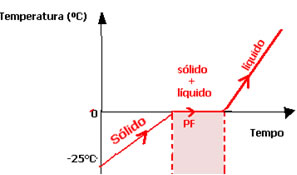
\includegraphics[width=0.5\textwidth]{gradico-do-ponto-de-fusao.jpg}
    \caption{Gráfico da temperatura da água pura em relação ao tempo.}
    \label{fig:solid_liquid}
\end{figure}

Perceba que durante o processo de fusão, \textbf{a temperatura do material se mantém constante, porque a energia dada para o material fundir é usada para a reorganização das moléculas e nada resta para aumentar a vibração das moléculas.} O mesmo é para caso o material esteja solidificando. A perda de energia não vem da diminuição da intensidade da vibração, mas sim da organização das moléculas.

Porém, para materiais que sejam misturas de compostos, como manteiga, isso não é verdade:

\begin{figure}[h]
    \centering
    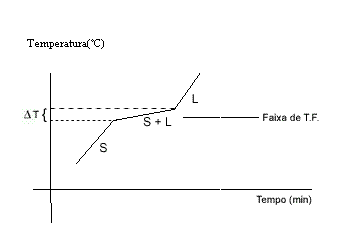
\includegraphics[width=0.5\textwidth]{fusao_irregular.png}
    \caption{Gráfico da temperatura de uma mistura em relação ao tempo.}
    \label{fig:azeotropic}
\end{figure}

Perceba que durante a mudança de estado, a temperatura continua a crescer e tem um $\Delta T$ entre o estado quando tudo é sólido para o quando tudo é líquido. \textbf{De forma simplificada, isso acontece quando os componentes das misturas de materiais possuem pontos de fusão distintos.} Dessa forma, quando um material da mistura está fundido, o outro ainda está sólido, ficando nessa mistura de estados até a temperatura que os dois materiais sejam líquidos.

\textbf{Isso também não é verdade para todas as misturas.} Cada mistura possui uma relação entre os seus componentes, de forma que uma mistura pode se comportar como uma substância pura (em que durante a fusão a temperatura é constante) ou como uma mistura (a temperatura durante a fusão não é constante).

\subsection{Ebulição e Liquefação}

Nesses processos é quando o material passa de líquido para gás ou vice-versa. Quando esse processo está ocorrendo, a vibração das moléculas quebram a atração entre as moléculas, tal que, agora, as moléculas passam a ocupar todo o espaço disponível (no estado líquido, elas se juntam e só ocupam um espaço determinado.) Para uma substância pura, o gráfico de temperatura por tempo para um material passando por essas transformações:

\begin{figure}[h]
    \centering
    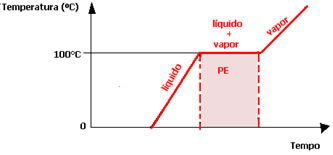
\includegraphics[width=0.5\textwidth]{gradico-do-ponto-de-ebulicao.jpg}
    \caption{Gráfico da temperatura em relação ao tempo para a água pura.}
    \label{fig:my_label}
\end{figure}

Novamente, quando começa a ocorrer o processo de fusão, a temperatura fica constante até que todo o líquido se transforme em gás, só então a temperatura volta a subir. \textbf{A explicação para isso é que durante esse processo, a energia dada a molécula é usada para quebrar a atração entre moléculas de forma que a vibração continua a mesma, logo a temperatura fica constante.}

Porém para materiais que sejam misturas de compostos, novamente o comportamento é outro:
\begin{figure}[H]
    \centering
    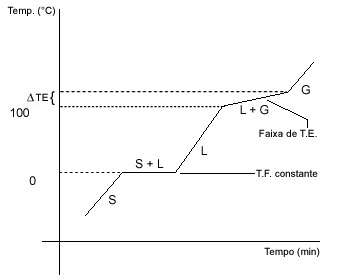
\includegraphics[width=0.5\textwidth]{ebulicao_irregular.jpg}
    \caption{Gráfico da temperatura por tempo de uma mistura.}
    \label{fig:mistura_ebulicao}
\end{figure}

Perceba que na transformação de líquido para gás, a temperatura continua a crescer. \textbf{Isso tem uma razão muito parecida com a anterior: a uma dada temperatura, acontece que uma substância da mistura já consegue quebrar a atração entre as moléculas, enquanto as outras substâncias ainda não conseguem, logo existe uma mistura de líquido com gás. Isso acaba quando todas as substâncias conseguem ebulir, logo a mistura vira completamente um gás.}

A mesma coisa vale para o caminho oposto, o da liquefação.

\subsection{Misturas especiais}
Existem algumas misturas que se comportam como substância pura no ponto de fusão ou de ebulição, mas no outro ponto, se comportam como mistura.

\begin{enumerate}
    \item \textbf{Mistura azeotrópica} - é quando a mistura se comporta como mistura no ponto de fusão, mas no ponto de ebulição se comporta como substância pura.
    
    \begin{figure}[H]
        \centering
        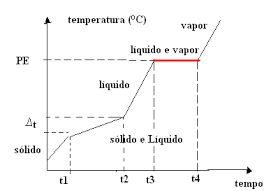
\includegraphics[width=0.5\textwidth]{download.png}
        \caption{Gráfico de temperatura por tempo de uma mistura azeotrópica}
        \label{fig:azeotropic}
    \end{figure}
    
    \item \textbf{Mistura eutética} - é quando a mistura possui se comporta como uma substância pura no ponto de fusão, mas no ponto de ebulição se comporta como uma mistura. O gráfico da figura (\ref{fig:mistura_ebulicao}) é de uma mistura eutética.
    
    \subsection{Sublimação}
    
    É quando acontece uma transformação de sólido para gás, diretamente, sem passar pela fase líquida. Isso acontece para certos materiais como a naftalina. O gráfico é semelhante aos apresentados, em que os estados são o sólido e o gasoso.
    
    \section{Diagrama de Estados (Fases)}
    
    Uma questão importante a mudança de fase é saber quando ocorre uma. Desde o século 18-19, percebeu-se que 2 quantidades ditam as mudanças de estados: \textbf{a pressão (P) e a temperatura (T)}. 
    
    Com isso, começou-se a mexer nessas quantidade para verificar o quanto elas mudavam os estados e poder mapear o comportamento dos materiais. O principal deles é o da água:
    
    \begin{figure}[H]
        \centering
        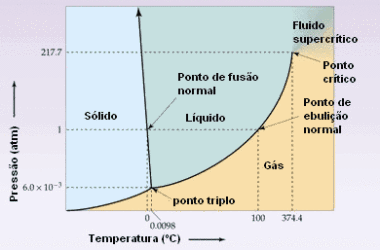
\includegraphics[width=0.8\textwidth]{diagrama-agua.png}
        \caption{Diagrama de estados/fases da água para a pressão em relação à temperatura}
        \label{fig:phase_diagram}
    \end{figure}
    
    A forma como você cruza a fronteira é o processo que acontece. Por exemplo: se você cruza a fronteira de sólido para líquido, acontece a fusão. Se fizer o caminho inverso (de líquido para sólido), acontece a solidificação.
    
    Além disso, percebeu-se o caráter e a relação entre a temperatura e pressão. \textbf{Quanto maior a pressão, maior será a temperatura para ocorrer os processos e vice-versa.} O mais interessante disso, é que pode ocorrer que as fronteiras entre sólido e líquido, líquido e gás, sólido e gás se tocarem num ponto. Esse ponto é chamado de \textbf{ponto triplo}. Quando estamos sobre ele, a água se apresenta nos 3 estados, ou seja, existe gelo, água e vapor d'água.
    
    Só para a curiosidade, hoje consideramos que o diagrama de estados/fases da água é o seguinte (não cai no vestibular nada como esse gráfico a seguir):
    \begin{figure}[H]
        \centering
        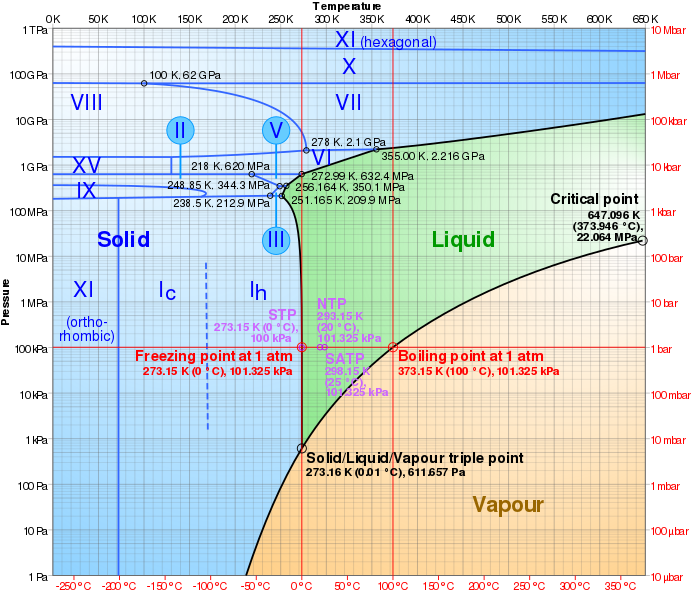
\includegraphics[width=0.8\textwidth]{700px-Phase_diagram_of_water.svg.png}
        \caption{Diagrama de fases da água mais atual. Hoje, consideramos que a água tem 11 estados distintos, a maioria é na forma sólida ("gelo").}
        \label{fig:my_label}
    \end{figure}
\end{enumerate}


\end{document}
